\documentclass[12pt]{article}  

\usepackage
[colorlinks=true, pdfstartview=FitV, linkcolor=blue, citecolor=blue, urlcolor=blue]
{hyperref}

\usepackage{amssymb}  
\usepackage{amsthm}
\usepackage{amsmath}
\usepackage{graphics} 
\usepackage{graphicx} 
%\usepackage[latin1]{inputenc}
\usepackage{tikz}
\usepackage{pgfplots}
\usepackage{wrapfig}
\usepackage{caption}
\usepgfplotslibrary{polar}
\usepackage{ skull }
\usetikzlibrary{decorations.fractals}


% GNUPLOT required
\usepackage{verbatim}

\linespread{1.3}

%\addtolength{\textwidth}{80pt}
\addtolength{\evensidemargin}{20pt}
\addtolength{\oddsidemargin}{20pt}

%%%%%%%%%%%%%%%%%%%%%%%%%%%%%%%%%%%%%%%%%%%%%%
%  Begin user defined commands

\newcommand{\map}[1]{\xrightarrow{#1}}

\newcommand{\N}{\mathbb N}
\newcommand{\Z}{\mathbb Z}
\newcommand{\Primes}{\mathbb P}
\newcommand{\Q}{\mathbb Q}
\newcommand{\R}{\mathbb R}
\newcommand{\C}{\mathbb C}
\newcommand{\bz}{\mathbb Z}
\newcommand{\bq}{\mathbb Q}
\newcommand{\br}{\mathbb R}
\newcommand{\bc}{\mathbb C}
\newcommand{\al}{\alpha}
\newcommand{\be}{\beta}
\newcommand{\ga}{\gamma}
\newcommand{\de}{\delta}
\newcommand{\ep}{\epsilon}
\DeclareMathOperator{\lub}{l.u.b.}
%  End user defined commands
%%%%%%%%%%%%%%%%%%%%%%%%%%%%%%%%%%%%%%%%%%%%%%


%%%%%%%%%%%%%%%%%%%%%%%%%%%%%%%%%%%%%%%%%%%%%%
% These establish different environments for stating Theorems, Lemmas, Remarks, etc.

\newtheorem{Thm}{Theorem}
\newtheorem{Prop}[Thm]{Proposition}
\newtheorem{Lem}[Thm]{Lemma}
\newtheorem{Cor}[Thm]{Corollary}

\theoremstyle{definition}
\newtheorem{Def}[Thm]{Definition}

\theoremstyle{remark}
\newtheorem{Rem}[Thm]{Remark}
\newtheorem{Ex}[Thm]{Example}

\theoremstyle{definition}
\newtheorem{Exercise}{Problem}

\newenvironment{Solution}{\noindent\textbf{Solution.}}{}

%\renewcommand{\labelenumi}{(\alph{enumi})}
\renewcommand\qedsymbol{QED}
% End environments 
%%%%%%%%%%%%%%%%%%%%%%%%%%%%%%%%%%%%%%%%%%%%%%%
%Some commands to save paper


\setlength{\parindent}{0in}
\setlength{\parskip}{8pt}

\DeclareMathOperator{\arcsec}{arcsec}
\DeclareMathOperator{\arccot}{arccot}
\DeclareMathOperator{\arccsc}{arccsc}
\DeclareMathOperator{\LH}{\ \underset{\text{LH}}{=}\ }
\newcommand{\Dep}{\Delta_+}
\newcommand{\Dem}{\Delta_-}
\newcommand{\bu}{\mathbf u}
\newcommand{\bv}{\mathbf v}
\newcommand{\bw}{\mathbf w}
\newcommand{\bx}{\mathbf x}

\newcommand{\ora}{\overrightarrow}



\addtolength{\textwidth}{80pt}
\addtolength{\evensidemargin}{-40pt}
\addtolength{\oddsidemargin}{-40pt}
\addtolength{\topmargin}{-80pt}
\addtolength{\textheight}{1.8in}

\setlength{\parindent}{0in}
\setlength{\parskip}{8pt}

\DeclareMathOperator{\arcsinh}{arcsinh}

%%%%%%%%%%%%%%%%%%%%%%%%%%%%%%%%%%%%%%%%%%%%%%
% Now we're ready to start
%%%%%%%%%%%%%%%%%%%%%%%%%%%%%%%%%%%%%%%%%%%%%%

\begin{document}  

%\author{Your Name}
{\bf MATH 1103 Homework 7}\\
{\bf Due Friday March 23, 2018}

%Practice Problems (not to be turned in)

%{\bf Practice 1.\ } 
%{\bf Practice 2.\ } 
%{\bf Practice 3.\ } 
%{\bf Practice 4.\ }   \rule{\textwidth}{1pt}
%The homework to be turned in may be found on the next page.




{\bf Homework 7 problems to be turned in.}

{\bf 1.\ } The purpose of this problem is to give some justification for Wallis and Cavalieri's idea that the area of a figure is a ``sum of lines".  Consider a monotone figure, as in Newton's Lemma II, over the interval $[0,1]$. Divide the base into $n$ equally spaced points $\frac{0}{n}, \frac{1}{n}, \dots, \frac{n-1}{n}$ and let $A_n$ be the the average length of the vertical lines within the figure above these points. The picture shows the case $n=4$. 

\begin{center}
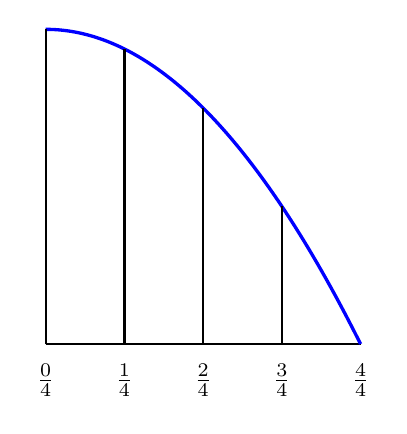
\begin{tikzpicture}[samples=100, domain=0:4, scale=1,
declare function = {f(\x) =4-(1/4)*\x*\x;}]]
\draw[black,   thick] (0,0) -- (4,0 );
\draw[blue, very thick] plot [domain=0: 4 ] (\x,{f(\x)}) ;
\draw[black,   thick] (0,0) -- (0,{f(0)} );
\draw[black,   thick] (1,0) -- (1,{f(1)} );
\draw[black,   thick] (2,0) -- (2,{f(2) });
\draw[black,   thick] (3,0) -- (3,{f(3)} );
\draw[black,   thick] (4,0) -- (4,{f(4)} );
 \node[label=below: {$\frac{0}{4}$}] at (0,0) {};
 \node[label=below: {$\frac{1}{4}$}] at (1,0) {};
 \node[label=below: {$\frac{2}{4}$}] at (2,0) {};
 \node[label=below: {$\frac{3}{4}$}] at (3,0) {};
 \node[label=below: {$\frac{4}{4}$}] at (4,0) {};
\end{tikzpicture}
\end{center}

Show that the area of the figure equals $\lim\limits_{n\to \infty}A_n$. 



{\bf 2.\ } Legend has it that when Gauss was in elementary school his teacher tried to punish the class by making them add up the integers from 1 to 100. How annoying then, when little Gauss did it in a few seconds, in his head. Can you? In any case, find a polynomial  function $G(x)$ such that  
$G(x)=\sum\limits_{k=1}^n k$. You will use the function $G(x)$ in the next three problems. 


\vskip10pt 
{\bf 3.\ } Compute $\sum\limits_{k=1}^n k^3$ for various small integers $n$, and make a conjecture relating this sum to $G(x)$. This formula is attributed to  {\bf Nichomachus}, from the first century AD. 

\vskip10pt 

{\bf 4.\ } Let $f(x)=x$ on the interval $[0,1]$, take an integer $n$, and let  $\bx$ be the partition of $[0,1]$ into $n$ equal parts.  

a)\ Compute $L(f,\bx)$ and $U(f,\bx)$ in terms of the function $G(x)$ from problem 1. Then let $n\to \infty$ to compute the area under the graph of $f$ (the hard way).  

b)\ Repeat part a) for the function $f(x)=x^3$, using Nichomachus' formula from problem 2.  Verify that Fermat gives the same answer (see hw 2). 



\vskip10pt 
{\bf 5.\ } Given any real number, let $\lfloor x \rfloor$ be the largest integer $\leq x$. The function $f(x)=\lfloor x \rfloor$ is called the {\bf floor function}. 

a)\ Graph the  function $f(x)=\lfloor x\rfloor$. 

b)\ Compute $L(f,\bx)$ and $U(f,\bx)$ where  $\bx$ is the fair partition of the interval $[0,4]$ into $8$ equal parts. 

c)\ Compute $L(f,\bx)$ and $U(f,\bx)$ where  $\bx$ is the fair partition of the interval $[0,4]$ into $4n$ equal parts, where $n$ is any positive integer. Verify that $U-L$ is the area of the tallest rectangle, as in Newton's proof of Lemma II. 

d)\ Use your answer to c) to compute $\int_0^4 f$. 


\end{document}








 
 
